\documentclass[UTF8]{ctexart}
\usepackage{bm}
\usepackage{amssymb}
\usepackage{mathtools}
\usepackage{amsmath}
\usepackage{float}
\usepackage{rotating}
\usepackage{booktabs}
\usepackage{pdfpages}

\title{\heiti 最优化第十一次作业}
\author{\kaishu 张晋15091060}
\begin{document}
\maketitle
\begin{enumerate}
\item[5.3]
\begin{enumerate}
\item 
\begin{equation}
\text{设}\quad q(\bm{x})=\dfrac{1}{2}\bm{x}^TG\bm{x}-\bm{b}\bm{x}
\end{equation}

由题意可知:
\begin{align}
\nabla q( \bm{x}) &=\bm{g}(\bm{x}) =G\bm{x}-\bm{b}\\
\nabla^{2}\bm{q}\left( \bm{x}\right)&=G\\
G\bm{s}&=\lambda \bm{s}
\end{align}



\begin{align}
\bm{g}(\bm{x}^{(0)})&=\bm{g}^{(0)}=G\bm{x}^{(0)}-\bm{b}\\
\bm{g}(\bm{x}^{(\star)})&=\bm{g}^{\star}=G\bm{x}^{\star}-\bm{b}=\bm{0}\\
\bm{g}^{(0)}&=\bm{g}^{(0)}-\bm{g}^{(\star)}=G(\bm{x}^{(0)}-\bm{x}^{\star})=G\mu\bm{s}=\mu\lambda\bm{s}
\end{align}


\begin{align}
\bm{x}^{(1)}&=\bm{x}^{(0)}-\dfrac{{-{\bm{g}^{(0)}}^T}\bm{g}^{(0)}}{{\bm{g}^{(0)}}^T\bm{G}\bm{g}^{(0)}}\\
&=\bm{x}^{(0)}-\dfrac {\mu^{2}\lambda^{2}\bm{s}^{T}\bm{s}}{\mu^{2}\lambda^{2}\lambda \bm{s}^{T}\bm{s}}\mu\lambda\bm{s}\\
&=\bm{x}^{(0)}-\mu\bm{s}\\
&=\bm{x}^{\star}
\end{align}

\item 
若$G=\lambda \bm{I}$,则对于$\bm{x}^{(0)}-\bm{x}^{\star}=\lambda \bm{t}$,易见$\bm{t}$为$G$相对于$\lambda $的特征向量,由(1)可知对任意的初始点$\bm{x}^{(0)}$,其沿最速下降方向进行一次精确线搜索后达到最优解

\item 
\begin{align}
g^{(0)}&=G\left( x^{(0)}-x^{\ast }\right)\\
&=G\sum ^{m}_{i=1}\mu _{i}\bm{s}_{i}\\
&=\sum ^{m}_{i=1}\mu _{i}\lambda _{i}\bm{s}_{i}
\end{align}


\begin{align}
\bm{x}^{(1)}&=\bm{x}^{(0)}-\dfrac{{-{\bm{g}^{(0)}}^T}\bm{g}^{(0)}}{{\bm{g}^{(0)}}^T\bm{G}\bm{g}^{(0)}}\\
&=\bm{x}^{(0)}-\dfrac {\sum ^{m}_{1=1}\sum ^{m}_{j=1}\mu _{i}\mu _{j}\lambda_{i}\lambda_{j}\bm{s}^{T}_{i}\bm{s}_{i}}{\sum ^{m}_{1=1}\sum ^{m}_{j=1}\mu _{i}\mu _{j}\lambda_{i}\lambda_{j}^2\bm{s}^{T}_{i}\bm{s}_{i}}\sum ^{m}_{i=1}\mu _{i}\lambda _{i}s_{i}\\
&=\bm{x}^{(0)}-\dfrac {\sum ^{m}_{1=1}\mu _{i}^2\lambda_{i}^2\bm{s}^{T}_{i}\bm{s}_{i}}{\sum ^{m}_{1=1}\mu _{i}^2\lambda_{i}^3\bm{s}^{T}_{i}\bm{s}_{i}}\sum ^{m}_{i=1}\mu _{i}\lambda _{i}\bm{s}_{i}\\
&=\bm{x}^{(0)}-\left( \sum ^{m}_{i=1}\dfrac {1}{\lambda _{i}}\right) \left(
\sum ^{m}_{i=1}\mu _{i}\lambda _{i}\bm{s}_{i}\right) 
\end{align}


\begin{align}
G\bm{x}^{(1)}-\bm{b}
&=G x^{(1)}-G x^{(0)}\\
&=G (x^{(1)}- x^{(0)})\\
&=-G\left( \sum ^{m}_{i=1}\dfrac {1}{\lambda _{i}}\right) \left(
\sum ^{m}_{i=1}\mu _{i}\lambda _{i}\bm{s}_{i}\right) \\
&=\left( \sum ^{m}_{i=1}\dfrac {1}{\lambda _{i}}\right) \left(
\sum ^{m}_{i=1}\mu _{i}\lambda _{i}^2\bm{s}_{i}\right) 
\end{align}
由于$\bm{s}_i$线性无关,故式(22)必然不等于0,即证
\end{enumerate}

\item[5.4]由于其为精确线搜索,故有:$\nabla f\left( x^{\left( k+1\right) }\right)^{T}p\left( k\right) =0
$,即$\bm{g}^{{(k+1)}^T}\bm{p}^{(k)}=-\bm{p}^{(k+1)^T}\bm{p}^{(k)}=0$

\[G=\begin{bmatrix}
20&0\\
0&2
\end{bmatrix}\]
得$\lambda_1=20,\lambda_2=2,\quad (\dfrac {\lambda_{1}-\lambda_{n}}{\lambda_{1}+x_{n}})^2 =81/121=0.66942$

\begin{figure}[H]
\small
\centering
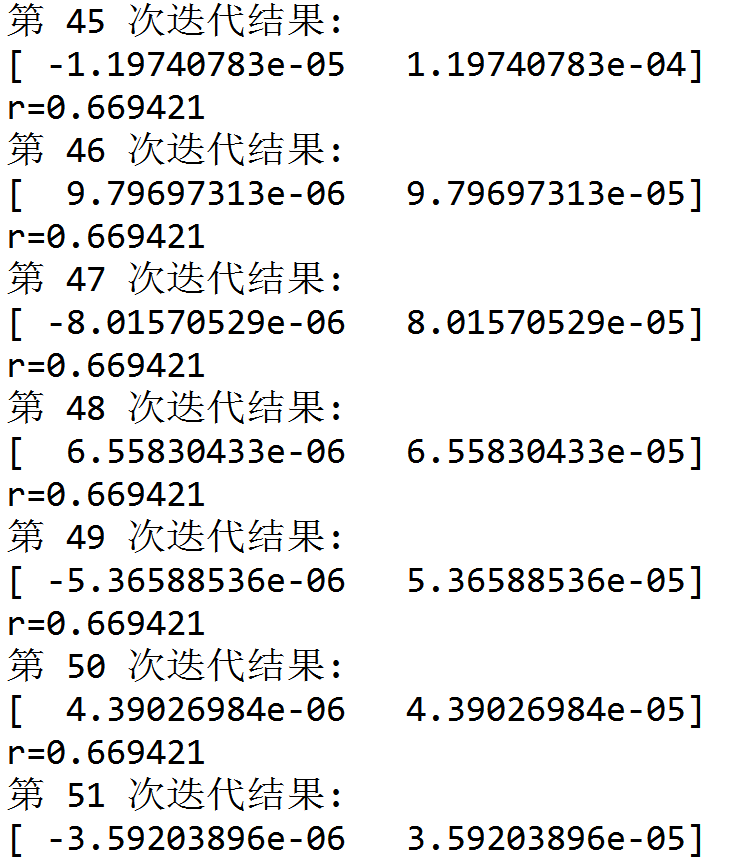
\includegraphics[width=6cm]{1.png}
\caption{输出}
\end{figure}

\begin{figure}[H]
\small
\centering
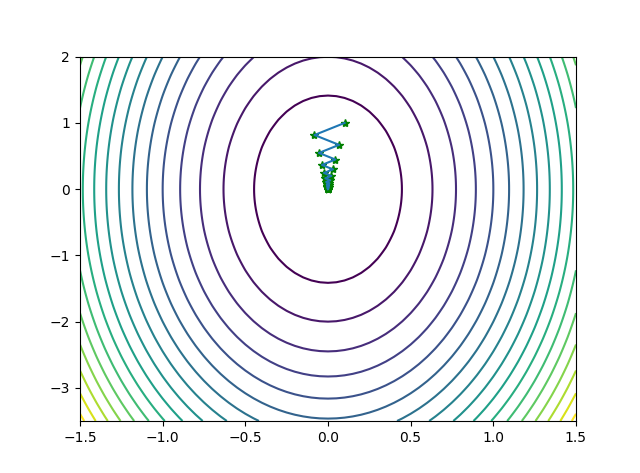
\includegraphics[width=10cm]{2.png}
\caption{图像}
\end{figure}

\item[5.6]
\[G=\begin{bmatrix}
10&-9\\
-9&10
\end{bmatrix},\qquad \lambda_1=19,\lambda_2=1,(\dfrac {\lambda_{1}-\lambda_{2}}{\lambda_{1}+x_{2}})^2 =0.81\]

\begin{figure}[H]
\small
\centering
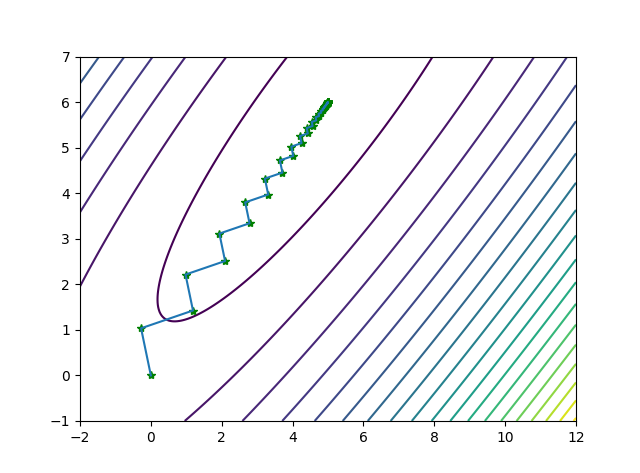
\includegraphics[width=10cm]{3.png}
\caption{初始点为$(0,0)$的图像}
\end{figure}

\begin{figure}[H]
\small
\centering
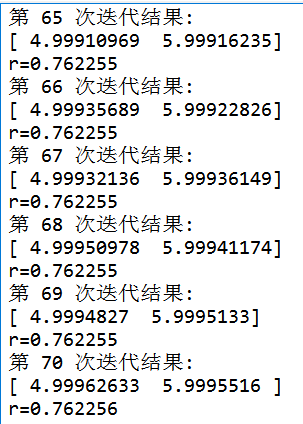
\includegraphics[width=6cm]{4.png}
\caption{初始点为$(0,0)$的输出}
\end{figure}

\begin{figure}[H]
\small
\centering
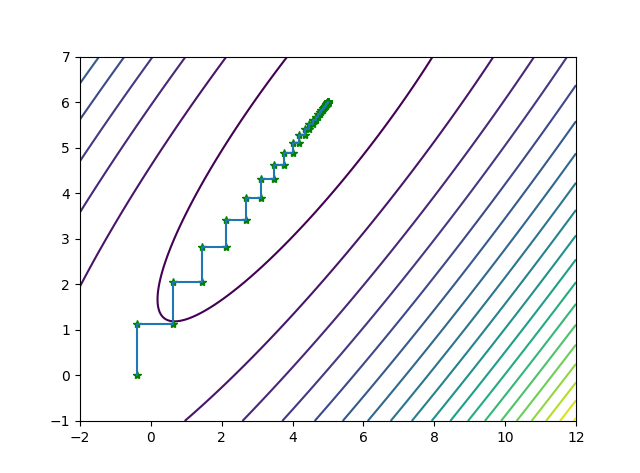
\includegraphics[width=10cm]{5.png}
\caption{初始点为$(-0.4,0)$的图像}
\end{figure}

\begin{figure}[H]
\small
\centering
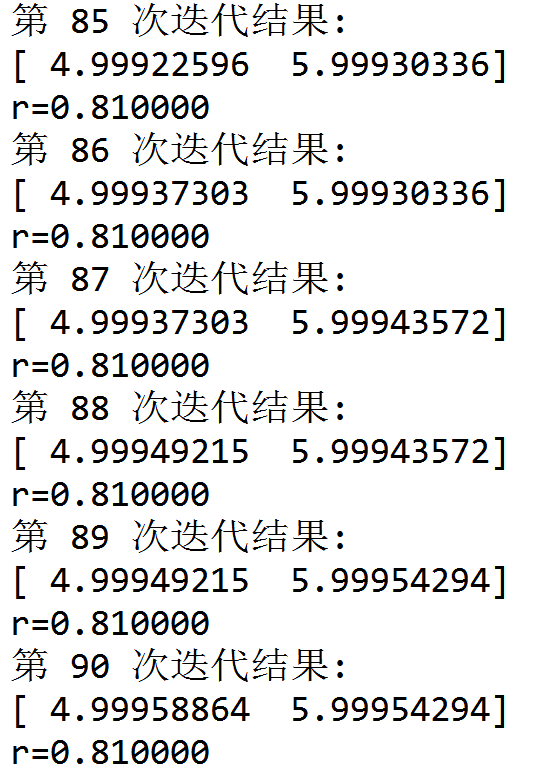
\includegraphics[width=6cm]{6.png}
\caption{初始点为$(-0.4,0)$的输出}
\end{figure}

\begin{figure}[H]
\small
\centering
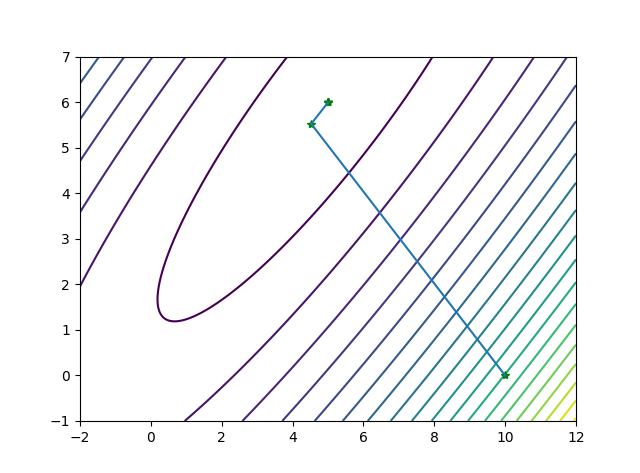
\includegraphics[width=10cm]{7.png}
\caption{初始点为$(10,0)$的图像}
\end{figure}

\begin{figure}[H]
\small
\centering
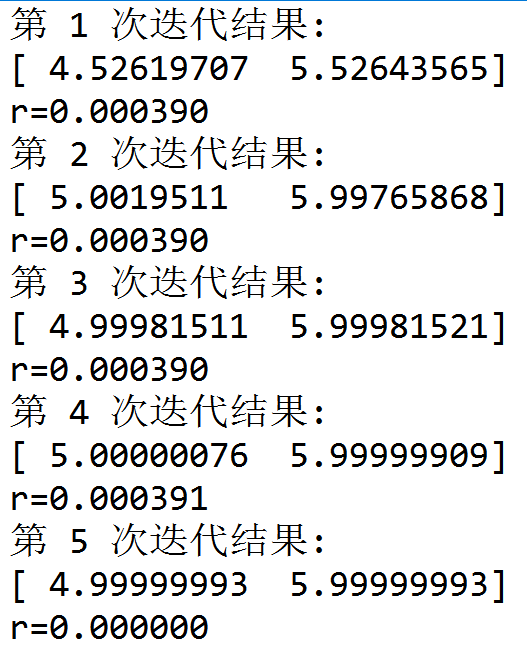
\includegraphics[width=6cm]{8.png}
\caption{初始点为$(10,0)$的输出}
\end{figure}

\begin{figure}[H]
\small
\centering
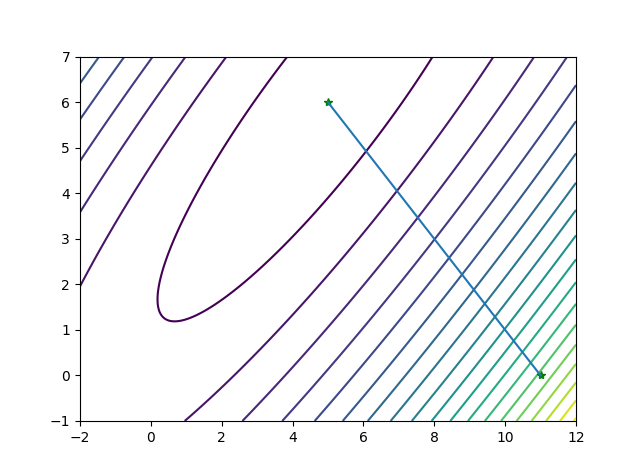
\includegraphics[width=10cm]{9.png}
\caption{初始点为$(11,0)$的图像}
\end{figure}

\begin{figure}[H]
\small
\centering
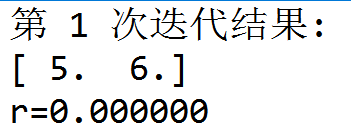
\includegraphics[width=6cm]{10.png}
\caption{初始点为$(11,0)$的输出}
\end{figure}

综上:第三次迭代时取到序列极限最大值0.81,根据计算此即是线性收敛因子。

\newpage
\item[5.11]
\[f({x},{y})\text{:=}\frac{1}{2} \left(x^2+y^2\right) e^{x^2-y^2}\]
\[\nabla _{\{x,y\}}f(x,y)=\left[x e^{x^2-y^2}+x e^{x^2-y^2} \left(x^2+y^2\right),y e^{x^2-y^2}-y e^{x^2-y^2} \left(x^2+y^2\right)\right]^T\]

\begin{equation}
\begin{bmatrix}
\dfrac {\partial ^{2}f}{\partial x^{2}}\\
\dfrac {\partial ^{2}f}{\partial x\partial y}\\
\dfrac {\partial ^{2}f}{\partial y^{2}}
\end{bmatrix}
=
\begin{bmatrix}
 4 e^{x^2-y^2} x^2+2 e^{x^2-y^2} \left(x^2+y^2\right) x^2+e^{x^2-y^2}+e^{x^2-y^2} \left(x^2+y^2\right) \\ 
 -2 e^{x^2-y^2} x y \left(x^2+y^2\right) \\ -4 e^{x^2-y^2} y^2+2 e^{x^2-y^2} \left(x^2+y^2\right) y^2+e^{x^2-y^2}-e^{x^2-y^2} \left(x^2+y^2\right)\end{bmatrix}
 \end{equation}

对于点$(0,0)^T$,有:
\[\nabla _{\{0,0\}}f(x,y)=[0,0]^T\]
\[G(0,0)=\begin{bmatrix}
1&0\\
0&1
\end{bmatrix}\]
故其是局部极小点。

对于点$(1,1)^T$,有:
\[\nabla _{\{1,1\}}f(x,y)=[0,0]^T\]
\[G'=G(1,1)=\begin{bmatrix}
11&-4\\
-4&-1
\end{bmatrix}\]
故其Hessian非正定.
显然$\lambda=3$是使得$G'+\lambda \bm{I}$正定的最小整数
由于$\nabla _{\{1,1\}}f(x,y)=\bm{0}$,故$\bm{s}=0,\quad \bm{x}''=\bm{x}'=(1,1)^T$

\end{enumerate}
\end{document}
